\newpage
\section{Auswertung}
\label{sec:auswertung}

Bei den folgenden Messauswertungen wurde ein Fehler von $\sqrt{N}$ bei $N$ gemessenen Ereignissen pro Kanal verrechnet, da diese Poisson verteilt sind.
Für alle \textit{fits}, die in der Auswertung vorkommen, wurde das \textit{python} Packet \textit{LMFIT} verwendet\cite{lmfit}.

\subsection{Halbwertsbreite bei variierender Verzögerung}
Es wurden für die Bestimmung der Halbwertsbreite, auch \enquote{full width at half maximum}, kurz fwhm, genannt, eine Verzögerung von je \SI{15}{\nano\second} bei beiden Verzögerungsleitungen eingestellt.
Daraus ergibt sich eine Verzögerungsdifferenz zwischen den beiden Leitungen zwischen -\SI{15}{\nano\second} und \SI{15}{\nano\second}.\\
Bei einem Messintervall von $\Delta t = \SI{10}{\second}$ werden die Pulse der PMTs gezählt und gegen die Verzögerungsdifferenz aufgetragen, was in \autoref{fig:fwhm} zu sehen ist.

\begin{figure}[H]
    \centering
    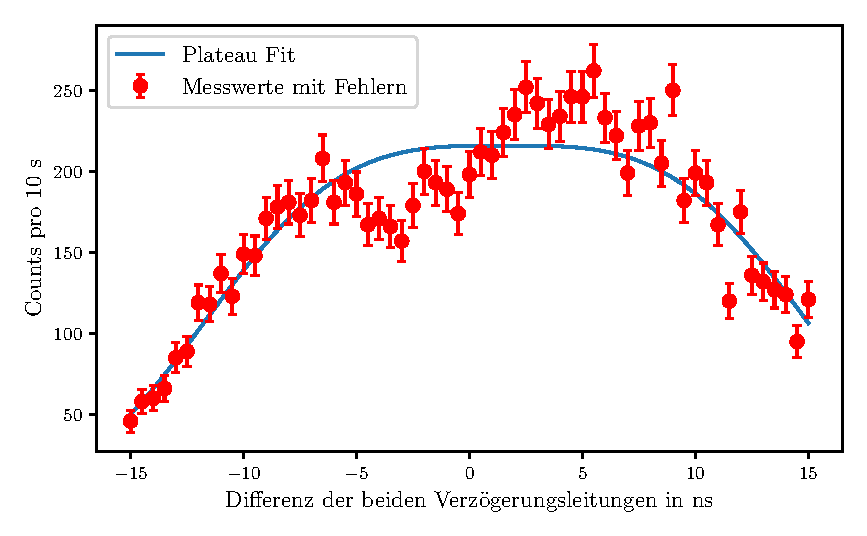
\includegraphics{images/fwhm.pdf}
    \caption{Gezählte Pulse bei verschiedenen Verzögerungseinstellungen der Verzögerungsleitungen, sowie ein Fit zur Annäherung des Verlaufs und zur Bestimmung des fwhm.}
    \label{fig:fwhm}
\end{figure}

Wie in \autoref{sec:durchfuerung} beschrieben, gibt die Koinzidenz nur ein Signal aus, wenn beide PMT einen Lichtblitz messen.
Wird die Messung eines PMT zu stark verzögert, so gibt es kein Signal.\\
Zu erwarten ist somit eine Plateaufunktion mit seitlich abfallenden Werten und dem Plateau dazwischen.
Zur Bestimmung der Halbwertsbreite wurde der Verlauf der Messdaten an eine Plateau-Funktion angenähert.
In \autoref{fig:fwhm} ist dieser Plateau-Fit dargestellt, dessen Funktionsparameter berechnet wurden zu:
\begin{itemize}
    \item $A = 215.914$
    \item $\mu = 1.617$
    \item $\sigma = 14.843$
    \item $n = 1.675$
\end{itemize}
bei einer Plateau-Funktion der Form
\begin{equation}
    f(x;A,\mu,\sigma, n) = A\cdot \exp\left(-\left(\frac{\left|x - \mu\right|}{\sigma}\right)^{2n}\right)
\end{equation}.\\
Die Halbwertsbreite lässt sich aus den Werten des Minimums und des Plateaus ermitteln.
Der halbe Wert beträgt $82.877\pm0.007$ counts und ergibt eine Breite von $fwhm = \left(29.305\pm0.0014\right)\si{\nano\second}$.\\
Die Daten sind in \autoref{tab:fwhm} aufgelistet.

\subsection{MCA Kalibration}
\label{sec:calli}
Für die Kalibration wurden die Pulsabstände von \SI{0.3}{\micro\second} schrittweise um \SI{0.5}{\micro\second} erhöht bis \SI{9.8}{\micro\second}.
Diese Pulsabstände werden gegen den Index der Kanäle des MCA aufgetragen, was in \autoref{fig:linear} dargestellt ist.

\begin{figure}[H]
    \centering
    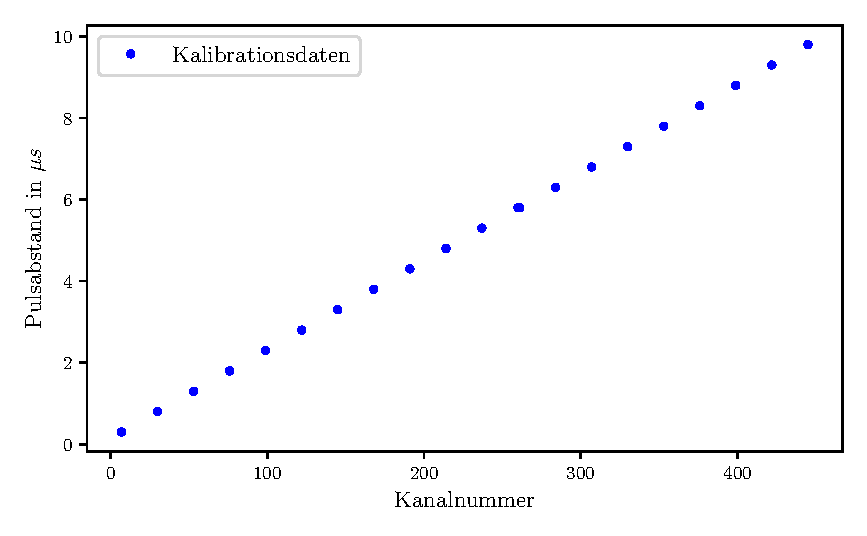
\includegraphics{images/linear.pdf}
    \caption{Abhängigkeit der Kanäle von dem Pulsabstand der Signale in \si[]{\micro\second}.}
    \label{fig:linear}
\end{figure}

Die Ausgleichsgerade ergibt eine Steigung von $0.0217\cfrac{\si{\micro\second}}{Kanal}$ und einen Startpunkt bei \SI{0.1542}{\micro\second}.
Die Funktion lautet somit
\begin{equation}
    f(x) = 0.0217x + 0.1542
\end{equation}
und gibt den jeweiligen Pulsabstand einer Kanalnummer an.\\
Die Daten sind in \autoref{tab:linear} aufgelistet.

\subsection{Berechnung der Untergrundrate}
Die Messung zeichnete 5635849 Start Signale auf und 15414 Stopp Signale.
Es gibt insgesamt 512 Kanäle, von denen die ersten vier sowie die letzten 47 keine Messdaten beinhalten.\\
Gemäß \autoref{eq:untergrund} wird zunächst der Erwartungswert der Verteilung $\lambda$ berechnet.
Die Suchzeit betrug $T_{\text{Such}} = $\SI{14}{\micro\second} und die totale Messzeit umfasste $t_{\text{ges}} = $\SI{253654}{\second}.
Daraus ergibt sich ein Erwartungswert von $\lambda \approx 311.06\cdot 10^{-6}$ und damit nach \autoref{eq:untergrund} ein Untergrund von $1752.55$.\\
Pro Kanal sind dies 3.423 Untergrundmessungen.

\subsection{Lebensdauer von Myonen}
In \autoref{fig:myonenroh} sind die rohen Messergebnisse nach ca. 3 Tagen totaler Messzeit in Abhängigkeit der Kanäle aufgetragen.

\begin{figure}[H]
    \centering
    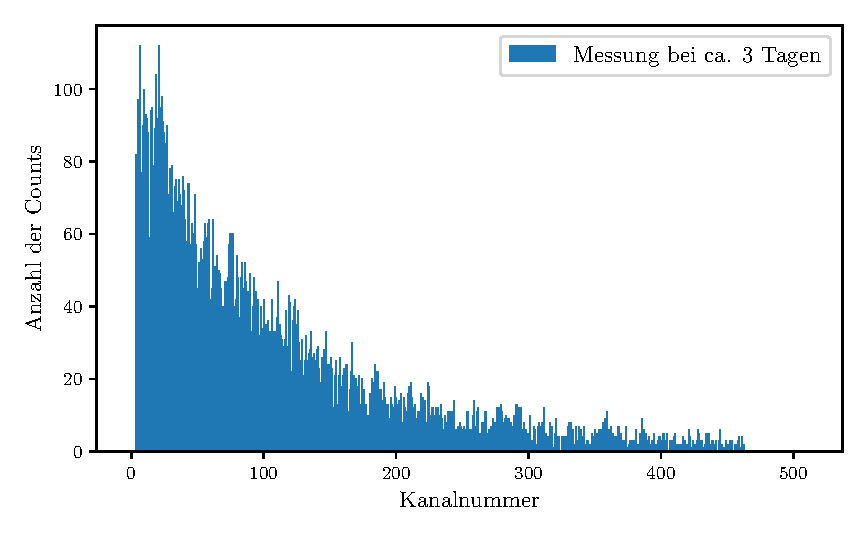
\includegraphics{images/messung_roh.pdf}
    \caption{Rohdaten nach ca. 3 Tagen Messung von Myonenlebensdauern.}
    \label{fig:myonenroh}
\end{figure}

Nach Konvertierung der Kanäle in Zerfallsdauern, mit der Ausgleichsgerade bestimmt in \autoref{sec:calli}, wird ein Fit an die Messdaten samt Unsicherheiten angelegt.
Das Ergebnis dieses Exponential-Funktion Fits, nach \autoref{eq:zerfall}, ist in \autoref{fig:myonen} dargestellt.
Hierbei wurden die Untergrundmessungen in den Unsicherheiten berücksichtigt und alle Nullwerte aus den Kanälen ohne Messwerte aus der Fit-Berechnung ausgelassen.

\begin{figure}[H]
    \centering
    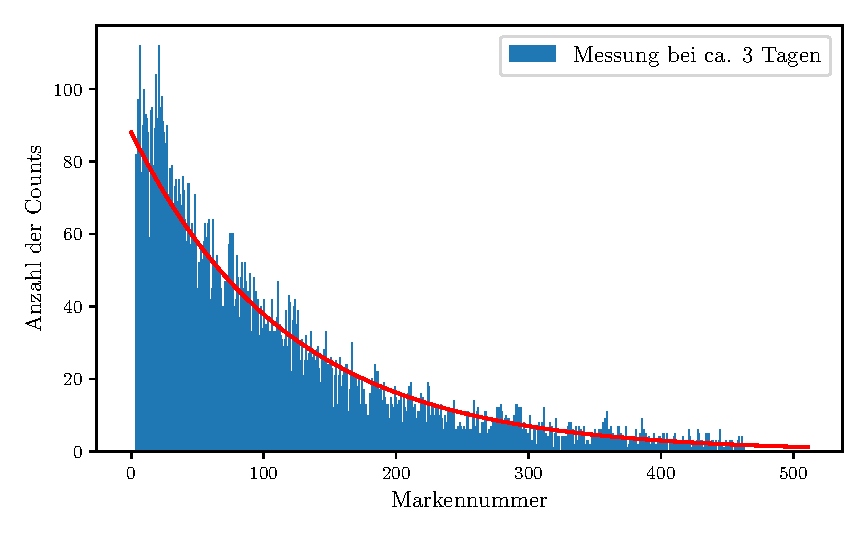
\includegraphics{images/messung_fit.pdf}
    \caption{Die Messdaten und der Fit der Messdaten samt Unsicherheiten sind gegen die Lebensdauer aufgetragen.}
    \label{fig:myonen}
\end{figure}

Die Fit-Parameter ergeben die Lebensdauer des Myons:
\begin{itemize}
    \item $N_0 = 93.6524 \pm 1.1433$
    \item $\tau = 2.5454 \pm 0.0417$\ \si{\micro\second}
\end{itemize}